\documentclass[11pt,a4paper]{article}
\usepackage[margin=2.5cm]{geometry}
\usepackage{graphicx}
\usepackage{hyperref}
\usepackage{amsmath}   % provides \operatorname, \text, etc.
\usepackage{amssymb}   % extra math symbols (if you happen to need them)

\usepackage{tikz}
\usetikzlibrary{arrows.meta, positioning, calc, decorations.pathreplacing}

\usepackage{bera}                   % optional: nicer monospaced font
\usepackage{listings}   % core
\usepackage{xcolor}     % colours for listings
\usepackage{newunicodechar} % ← lets you type “smart quotes”, →, … in code if needed

\usepackage{booktabs}
\usepackage{caption}
\usepackage{float}

\usepackage[dvipsnames]{xcolor}     % load lots of named colors
% define the JSON‐listing palette
\definecolor{background}{gray}{0.95}     % light grey background
\definecolor{string}{RGB}{42,0,255}      % blueish strings
\colorlet{punct}{red!60!black}           % punctuation
\definecolor{delim}{RGB}{20,105,176}     % braces/brackets
\colorlet{numb}{magenta!60!black}        % numbers

% ---------- GLOBAL STYLE ----------
\lstdefinestyle{code}{
  basicstyle=\ttfamily\small,
  columns=fullflexible,
  numbers=left,
  numberstyle=\tiny\color{gray},
  stepnumber=1,
  numbersep=6pt,
  breaklines=true,
  frame=single,
  framerule=0.2pt,
  rulecolor=\color{gray!60},
  tabsize=2,
  showstringspaces=false
}

% ---------- JSON ----------
\lstdefinelanguage{json}{
  style=code,
  literate=
   *{0}{{{\color{magenta}0}}}{1}
    {1}{{{\color{magenta}1}}}{1}
    {2}{{{\color{magenta}2}}}{1}
    {3}{{{\color{magenta}3}}}{1}
    {4}{{{\color{magenta}4}}}{1}
    {5}{{{\color{magenta}5}}}{1}
    {6}{{{\color{magenta}6}}}{1}
    {7}{{{\color{magenta}7}}}{1}
    {8}{{{\color{magenta}8}}}{1}
    {9}{{{\color{magenta}9}}}{1}
    {:}{{{\color{red}{:}}}}{1}
    {,}{{{\color{red}{,}}}}{1}
    {\{}{{{\color{blue}{\{}}}}{1}
    {\}}{{{\color{blue}{\}}}}}{1}
    {[}{{{\color{blue}{[}}}}{1}
    {]}{{{\color{blue}{]}}}}{1},
  morestring=[b]",
}

% ---------- Go ----------
\lstdefinelanguage{go}{
  style=code,
  keywords={break,case,chan,const,continue,default,defer,else,fallthrough,for,
            func,go,goto,if,import,interface,map,package,range,return,select,
            struct,switch,type,var},
  keywordstyle=\color{blue}\bfseries,
  ndkeywords={bool,byte,complex64,complex128,error,float32,float64,
              int,int8,int16,int32,int64,rune,string,uint,uint8,
              uint16,uint32,uint64,uintptr},
  ndkeywordstyle=\color{teal}\bfseries,
  morecomment=[l]{//},
  morecomment=[s]{/*}{*/},
  commentstyle=\color{gray}\itshape,
  morestring=[b]",
  stringstyle=\color{orange},
  sensitive=true
}

\hypersetup{
  colorlinks=true,
  linkcolor=blue,
  citecolor=blue,
  urlcolor=blue
}

\title{Peer-to-Peer File Sharing with BitTorrent\\
\large Course Project Report}
\author{Ivan Ch., Ksenia K., Anton K., Ilya O.}
\date{\today}

\begin{document}
\maketitle
\thispagestyle{empty}
\vspace*{\fill}
\begin{center}
\textbf{Abstract}\\[0.5em]
This report presents the design, implementation and evaluation of a simplified BitTorrent--style peer-to‑peer (P2P) file‑sharing system written in Go.  
The system implements chunked file transfer, rarest‑first piece selection, and decentralised peer discovery through a lightweight Distributed Hash Table (DHT).  
We validate our implementation on a local four‑node test‑bed and demonstrate successful end‑to‑end transfers without a central tracker.
\end{center}
\vspace*{\fill}
\clearpage

\tableofcontents
\clearpage

\section{Introduction}
BitTorrent popularised efficient P2P file distribution by splitting a file into many fixed‑size \emph{pieces} and exchanging them among peers in parallel.
Modern content delivery still relies on the same principles (e.g.\ WebTorrent, IPFS).
The aim of this project is to build a minimal yet functional BitTorrent‑like client from scratch in Go, focusing on
\begin{itemize}
  \item Decentralised peer discovery via a mini‑DHT (no tracker);
  \item Chunk exchange over TCP with rarest‑first scheduling;
  \item Structured JSON logging for observability.
\end{itemize}
We restrict ourselves to single‑file torrents and ignore advanced incentives (tit‑for‑tat) to stay within course scope.

\section{Background}\label{sec:background}
\subsection{BitTorrent Protocol}
The official BitTorrent specification\,\cite{bittorrent_spec} defines five core messages (\textsc{handshake}, \textsc{bitfield}, \textsc{request}, \textsc{piece}, \textsc{have}) exchanged over TCP after an initial handshake that carries the \emph{info‑hash}.
Peers maintain a \emph{bitfield} indicating which pieces they already possess.
\\ In our implementation, we also define such messages and handle them this way 

\begin{lstlisting}[language=go]
  func (peer *Peer) handle(message *protocol.Message) {
    if !peer.handshakeDone && message.ID != protocol.MsgHandshake {
        return
    }

    switch message.ID {
    case protocol.MsgHandshake:
        /* Compares expected hash and hash from handshake */ 

    case protocol.MsgBitfield:
        /* Receives the peer's available pieces bitfield */

    case protocol.MsgRequest:
        /* Peer requests a piece; server prepares and sends it */

    case protocol.MsgHave:
        /* Peer announces possession of a specific piece */

    case protocol.MsgPiece:
        /* Receives a piece of data and verifies its integrity*/
    }
}
\end{lstlisting}
No messages are accepted before the handshake is done

\subsection{Kademlia DHT}
Kademlia\,\cite{maymounkov2002kademlia} organises nodes in a 160‑bit XOR metric space and allows logarithmic‑time look‑ups.
Our DHT keeps the same bucket structure (\(k{=}8\)) but supports only three RPCs: \textsc{ping}/\textsc{pong}, \textsc{findPeers}, and \textsc{announce}.
\\ We handle RPC in such way:
\begin{lstlisting}[language=go]
  func (node *DHTNode) handle(msg Msg, adr *net.UDPAddr) {
    // Refresh routing table with sender's node-ID
    node.RoutingTable.Update(Peer{ID: id20, Addr: adr})

    switch msg.T {
    case "ping":
        // Receive ping request. 
        // Collect 10 peers from routing table.
        // Send pong with collected peers.

    case "pong":
        // Receive pong response and update routing table with new peers

    case "announce":
        // Register a TCP address for a given infohash in the seeds list

    case "findPeers":
        // Lookup and send known seeders for a requested infohash
    }
}  
\end{lstlisting}
-
\section{Simplified System Design}
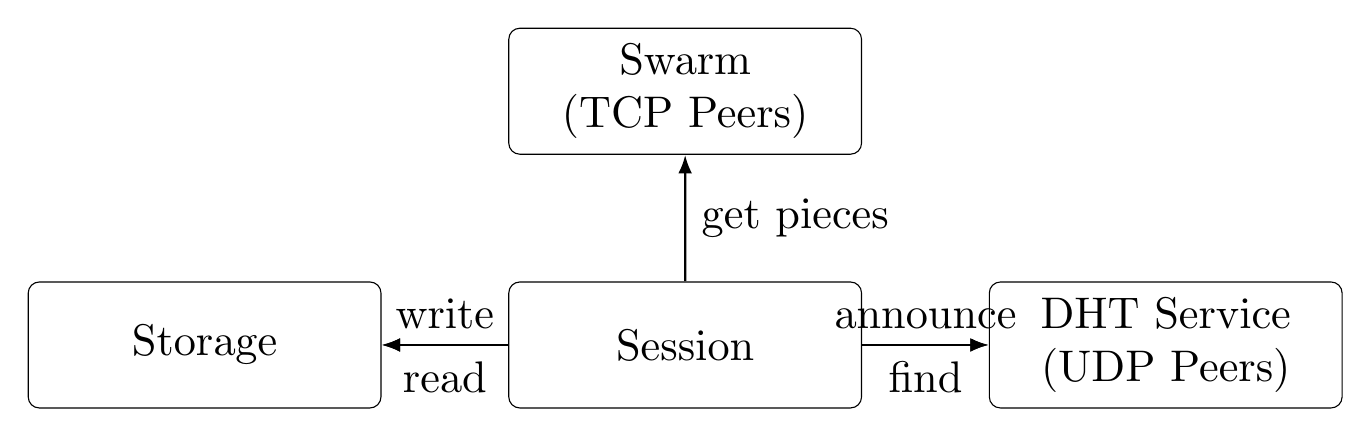
\begin{tikzpicture}[
  scale=1.6,                % <<—— adjust overall size here
  every node/.style={transform shape},
  node/.style={draw, rounded corners, minimum width=2.8cm, minimum height=1cm, align=center},
  arrow/.style={-{Latex}, thick}
]
  % Core orchestrator
  \node[node] (session) {Session};
  % Sub‑systems
  \node[node, above=of session]  (swarm)   {Swarm\\(TCP Peers)};
  \node[node, right=of session]  (dht)     {DHT Service\\(UDP Peers)};
  \node[node, left=of session]  (storage) {Storage};

  % Data / control flows
  \draw[arrow] (session) -- (swarm)   node[midway, right] {get pieces};
  \draw[arrow] (session) -- (dht)     node[midway, above] {announce};
  \draw[arrow] (session) -- (dht)     node[midway, below] {find};
  \draw[arrow] (session) -- (storage) node[midway, above] {write};
  \draw[arrow] (session) -- (storage) node[midway, below] {read};
\end{tikzpicture}

\newpage
\subsection{Concurrency Model}
The concurrency mechanisms of Go are extremely useful for the project.
Each outbound or inbound TCP connection runs two goroutines: a reader and a writer,
communicating with the rest of the program through a buffered channel 
of \texttt{protocol.Message}s:
\begin{lstlisting}[language=go]
  func New(conn net.Conn, bf storage.Bitfield, id, desiredInfohash [20]byte) *Peer {
    peer := &Peer{ ... }
    go peer.writer()
    go peer.reader()
    return peer
  }
  
  // Writes messages into connection
  func (peer *Peer) writer() {
    for msg := range peer.SendCh {
      msg.Encode(peer.Conn)
    }
  }
  
  // Reads messages from connection
  func (peer *Peer) reader() {
    for {
      peer.handle(protocol.Decode(peer.Conn))
    }
  }
\end{lstlisting}


The DHT runs its own UDP reader and a dispatcher goroutine.
\begin{lstlisting}[language=go]
  // Creates and start a new DHT node listening on a specified address.
  func New(listen string) (*DHTNode, error) {
    node := ...
    
    go node.udpLoop()      // Socket loop
    go node.dispatchLoop() // message handler
  
    return node, nil
  }  
  
\end{lstlisting}

\subsection{Data Structures}

\paragraph{Session} Owns every byte and handle that lives for the lifetime of \emph{one} `.bit` file — metadata, piece cache, peer swarm and optional DHT helper.
\begin{lstlisting}[language=go]
	type Session struct {
		// --- mutable ---
		Mu     sync.Mutex       // atomic piece writes
		Pieces [][]byte         // RAM cache of pieces
		BF     storage.Bitfield // pieces we own
		// --- constants ---
		InfoHash [20]byte
		Meta     *metainfo.Meta
		// --- subsystems ---
		DHT   *DHTService
		Swarm *Swarm
		cfg   *Config           // back-pointer to flags
	}
\end{lstlisting}

\paragraph{Swarm} Leecher-side brain that decides \emph{what} piece to ask \emph{which} peer (rarest-first) and announces completion.
\begin{lstlisting}[language=go]
	type Swarm struct {
		Sess  *Session      // shared buffers
		Peers []*peer.Peer  // active TCP conns
		// piece-picker state
		missing, availability []int
		ticker *time.Ticker
		destDir string
		keepSec int
	}
\end{lstlisting}

\paragraph{Peer} A goroutine pair (`reader` / `writer`) wrapping one TCP socket; pushes validated events upward to the swarm.
\begin{lstlisting}[language=go]
	type Peer struct {
		Conn     net.Conn
		Bitfield storage.Bitfield   // peer's inventory
		SendCh   chan protocol.Message
		Meta     *metainfo.Meta
		Pieces   [][]byte           // file pieces we have
		ID, RemoteID [20]byte
		OnHave   func(int)          // callback into Swarm
	}
\end{lstlisting}

\paragraph{DHTNode} A lightweight, JSON-encoded Kademlia actor that keeps a routing table, seeds map and two inboxes for UDP traffic.
\begin{lstlisting}[language=go]
	type DHTNode struct {
		ID   [20]byte
		Conn *net.UDPConn
		RoutingTable *dht.Table           // 160 buckets
		Seeds map[string][]string         // infoHash: []tcpAddr
		inbox, inboxPeer chan packet      // demuxed receives
	}
\end{lstlisting}

\paragraph{Msg} The \emph{only} packet that flies over UDP; optional fields let several RPCs share one wire format.
\begin{lstlisting}[language=go]
	type Msg struct {
		T        string   `json:"t"`              // "ping" | ...
		ID       string   `json:"id"`             // hex(nodeID)
		Info     string   `json:"info,omitempty"` // hex(infoHash)
		Addr     string   `json:"addr,omitempty"`
		TcpList  []string `json:"tcp_list,omitempty"`
		DHTPeers []MsgPeer`json:"dht_peers,omitempty"`
	}
\end{lstlisting}

\paragraph{Meta} A `.bit` manifest: file size, piece size and SHA-1 hash per piece (20 bytes each).
\begin{lstlisting}[language=go]
	type Meta struct {
		FileName   string   // base name of payload
		FileLength int64    // total bytes in payload
		PieceSize  int      // bytes per piece (256 KiB by default)
		Hashes     [][]byte // SHA-1 per piece
	}
\end{lstlisting}

\paragraph{Bitfield} A tiny compressed set that tells peers “I already own these pieces”.
\begin{lstlisting}[language=go]
	type Bitfield []byte // bf[i]==1 -> we have piece i
\end{lstlisting}

\paragraph{Message} Length-prefixed frames travelling on every TCP link; helper constructors create typed variants such as \texttt{NewRequest} or \texttt{NewPiece}.
\begin{lstlisting}[language=go]
	type Message struct {
		ID   uint8  // Handshake | Bitfield | Request | ...
		Data []byte // payload depends on ID
	}
\end{lstlisting}


\paragraph{Routing Table} A 160‑bucket Kademlia table.
Peers are evicted by least‑recently‑seen (LRU) once a bucket exceeds \(k=8\).
\begin{lstlisting}[language=go]
  type Table struct {
	  mu     sync.RWMutex
	  self   [20]byte
	  bucket [160]bucket
}
  
\end{lstlisting}

\newpage
\subsection{Piece Selection}
We implement \emph{rarest‑first}: every 2~s the leecher computes the availability of each still‑missing piece across known peers and requests the least replicated one.
\begin{lstlisting}[language=go]
  // Return rarest piece index by computing availability
  func (sw *Swarm) choosePiece() int {
    // Reset availability
    for i := range sw.availability {
      sw.availability[i] = 0
    }
  
    // Compare bitfields and recompute avail
    for _, p := range sw.Peers {
      for i := range sw.availability {
        if p.Bitfield.Has(i) {
          sw.availability[i]++
        }
      }
    }
  
    // Find rarest piece
    best := -1
    for i, need := range sw.missing {
      if !need { // No need to ask available piece
        continue
      }
      if best == -1 || sw.availability[i] < sw.availability[best] {
        best = i
      }
    }
    return best
  }  
\end{lstlisting}

%---------------- DHT ---------------------------------------------------------
\newpage
\subsection{DHT Table}\label{sec:dhttable}

\paragraph{Motivation.}
Efficient peer discovery requires each node to remember only a \emph{logarithmic}
view of the network.
Following Kademlia \cite{maymounkov2002kademlia} we partition the
160-bit XOR metric space into \(160\) \emph{\(k\)-buckets}; bucket \(b\)
collects peers whose IDs share exactly \(b\) leading bits with our own
\texttt{selfID}.
With a constant bucket capacity \(k{=}8\) this bounds memory to
\(k\!\times\!160 = 1280\) entries while still yielding
\(O(\log N)\) routing guarantees.

\paragraph{Core data structure.}
The implementation (\texttt{internal/dht/table.go}) stores buckets as
\lstinline[style=code]{[]Peer} slices guarded by an \lstinline{RWMutex}:

\begin{lstlisting}[language=go,caption={Routing-table excerpt (simplified).}]
const kSize = 8                     // bucket capacity

type Peer struct {
    ID   [20]byte
    Addr *net.UDPAddr
    Time time.Time                  // last seen
}

type bucket struct{ peers []Peer }

type Table struct {
    mu     sync.RWMutex
    self   [20]byte                 // this node's ID
    bucket [160]bucket              // one per prefix length
}
\end{lstlisting}

\paragraph{Insertion / refresh (\texttt{Update}).}
When a UDP packet is received the sender is added via
\lstinline{Table.Update}.  
The algorithm (Listing \ref{lst:update}) performs four
steps under a write lock:

\begin{enumerate}
  \item Ignore our own ID.
  \item Compute bucket index \(b = \operatorname{prefixLen}(ID \oplus selfID)\).
  \item Remove any previous occurrence of the peer (refresh).
  \item Append the peer as \emph{most-recent}; if the bucket now exceeds
        \(k\) entries the least-recent (LRU) element is evicted.
\end{enumerate}

\newpage
\begin{lstlisting}[language=go,caption={Peer refresh / LRU eviction},label={lst:update}]
func (t *Table) Update(p Peer) {
    if p.ID == t.self { return }                // 0. never store self
    b := prefixLen(xor(p.ID, t.self))           // 1. bucket index
    bk := &t.bucket[b]

    // 2. refresh: drop previous instance
    for i, q := range bk.peers {
        if q.ID == p.ID {
            bk.peers = slices.Delete(bk.peers, i, i+1)
            break
        }
    }

    // 3. append as MRU
    p.Time = time.Now()
    bk.peers = append(bk.peers, p)

    // 4. evict LRU if over capacity
    if len(bk.peers) > kSize {
        bk.peers = bk.peers[1:]
    }
}
\end{lstlisting}

\paragraph{Look-ups (\texttt{Closest}).}
Queries such as \textsc{findPeers} need the \emph{\(n\)} peers whose XOR
distance to a target key is minimal.
The routine first copies all bucket contents into a scratch slice,
then sorts it by
\(\mathit{dist}(a,b)=\text{bigInt}(a\oplus b)\) and returns the first
\(n\) entries:

\begin{lstlisting}[language=go,caption={Selecting the \(n\) closest peers.}]
func (t *Table) Closest(target [20]byte, n int) []Peer {
    t.mu.RLock(); defer t.mu.RUnlock()

    var cand []Peer
    for _, b := range t.bucket {
        cand = append(cand, b.peers...)
    }
    sort.Slice(cand, func(i, j int) bool {
        return dist(cand[i].ID, target).Cmp(
               dist(cand[j].ID, target)) < 0
    })
    if len(cand) > n { cand = cand[:n] }
    return cand
}
\end{lstlisting}

The overall complexity is
\(O(k\,\cdot160) = O(1)\) for
\texttt{Update}
and \(O(k\,160\log(k\,160))\approx O(10^4)\)
in the worst case for \texttt{Closest}, which is acceptable given the
small constant factor.

\paragraph{Concurrency considerations.}
Read-heavy operations (\texttt{Closest}) acquire only a shared
\lstinline{RLock}, allowing multiple look-ups to proceed in parallel,
while insertions use \lstinline{Lock} to guarantee LRU consistency.

\paragraph{Summary.}
This design keeps the
well-known asymptotic properties of Kademlia while remaining
implementation-friendly:

\begin{itemize}
  \item \textbf{Memory}: \( \le 1280 \) peers (\(160\) buckets × \(k{=}8\)).
  \item \textbf{Update}: constant-time LRU with mutex protection.
  \item \textbf{Query}: logarithmic network hops using
        \textsc{PING}/\textsc{FIND}\textsc{PEERS}.
\end{itemize}
It therefore provides a scalable yet lightweight substrate for the
tracker-less BitTorrent network used in this project.


\section{Protocol Details}
\subsection{TCP Messages}
\begin{table}[H]
\centering
\begin{tabular}{@{}llp{7cm}@{}}
\toprule
ID & Name & Payload \\ \midrule
0 & \textsc{handshake} & 20-byte infoHash \;+\; 20-byte peerID \\
1 & \textsc{bitfield} & N-byte (\(N{=}\) number of pieces) \\
2 & \textsc{request}  & 4-byte piece‑index \;+\; 4-byte offset (\(0\)) \\
3 & \textsc{piece}    & 4-byte piece‑index \;+\; 4-byte offset \;+\; N-bytes data \\
4 & \textsc{have}     & 4-byte piece‑index \\ \bottomrule
\end{tabular}
\caption{Implemented TCP message types.}
\end{table}

\subsection{UDP DHT Messages}
\textsc{ping}, \textsc{pong}, \textsc{announce}, \textsc{findPeers}, \textsc{peers};
\\ All serialised as JSON for readability and convenience (see \texttt{internal/dht/msg.go}).

\section{Implementation Highlights}
\begin{itemize}
  \item \textbf{Logger}: thread‑safe structured JSON, allowing real‑time inspection via \texttt{jq}.
  \item \textbf{Session}: owns per‑torrent state (\texttt{Meta}, in‑memory pieces, bitfield, DHT service, swarm).
  \item \textbf{Swarm}: orchestrates piece requests and maintains peer list.
  \item \textbf{Safety}: verified with Go race detector; no data races found.
\end{itemize}

\section{Experiments \& Results}
\subsection{Use Cases}
Let's open four terminal and launch our torrent client there. Before diving into the experiment,
let us explain the configuration flags

% func ParseFlags() *Config {
% 	var c Config
% 	flag.IntVar(&c.KeepSeedingSec, "keep", 0, "seconds to keep seeding after complete")
% 	flag.Parse()
% 	return &c
% }

\begin{enumerate}
  \item \textbf{-tcp-listen N} - specify address N for tcp listening. Seeders will listen for requests on this port
  \item \textbf{-dht-listen N} - specify address N for udp listening. Every network node needs this.
  \item \textbf{-bootstrap N,M,X} - specify udp addresses N,M,X (csv) for system bootstrapping. Without bootstrapping node will never reach the network, so one have to provide at least one node there
  \item \textbf{-peer N,M,X} - specify tcp addresses N,M,X for udp listening. Not really needed if you specified some good UDP node, that will tell you about seeders. However, you might use it if you are not interested in UDP testing and you want to go straight to pieces exchange testing
  \item \textbf{-seed path/to/file} - AS A SEEDER specify the filepath you want to seed. The file.bit (metadata) will be produced in the same directory as the file you seeded.
  \item \textbf{-get path/to/file.bit} - AS A LEECHER specify filepath of .bit file (metadata).
  \item \textbf{-dest download/file/to} - AS A LEECHER specify filepath where you desire to download seeded file.
  \item \textbf{-keep N} - AS A LEECHER specify seconds amount you desire to seed after getting the file.
\end{enumerate}
I also use \textbf{"| jq ."} so json logs are formatted pretty.
Also I will refer to terminals 1-2-3-4 just by number.

\vspace{4mm} Let the first terminal have the role of simple DHT-node, without seeding or leeching abilities.
\begin{lstlisting}[language=go]
go run ./cmd/bittorrent -dht-listen :10000 -tcp-listen :10001 | jq .
\end{lstlisting}
It will launch dht-node on localhost:10000 for udp, localhost:10001 for tcp. It is going to wait for nodes to connect.

\vspace{4mm} Second terminal will have the role of seeder and will seed 524MB movie
\begin{lstlisting}[language=go]
go run ./cmd/bittorrent -seed ~/Documents/lenses_presentation.mov -bootstrap :10000 -tcp-listen :20001 -dht-listen :20000 | jq .
\end{lstlisting}
I added flags -bootstrap in order to connect seeder and 1-node and -seed to seed the file.
After running, one should expect to see the following two cases.
\begin{enumerate}
  \item Everything worked fine (usually). DHT and Seeder connected. Following logs produced on seeder side (besides other ones) \begin{lstlisting}[language=json]
{
  "event": "udp_send",
  "size": 130,
  "to": "127.0.0.1:10000",
  "ts": "2025-04-27T15:13:31.334306Z",
  "type": "announce"
}

{
  "event": "seeder_ready",
  "file": "/Users/ivanchabanov/Documents/lenses_presentation.mov",
  "infoHash": "904a09802b66917501f8cb5ce31c340fad128da0",
  "tcp": ":20001",
  "ts": "2025-04-27T15:13:31.33604Z"
}
\end{lstlisting}
\item You started seeder earlier and it sent ping not to DHT but networks darkness. This case you will never catch with DHT-node \begin{lstlisting}[language=json]
{
  "event": "seeder did not find DHT yet... try again after 5 sec",
  "ts": "2025-04-27T15:35:37.793721Z"
}
\end{lstlisting}
\end{enumerate}

\vspace{8mm} Third terminal will be a leecher. Also keep it for 20 minutes to seed (-keep 1200).
\begin{lstlisting}[language=go]
  go run ./cmd/bittorrent -get ~/Documents/lenses_presentation.mov.bit  -bootstrap :10000 -dht-listen :30000  -tcp-listen :30001 -keep 1200 | jq .
\end{lstlisting}
\begin{enumerate}
  \item After booting, leecher will ping-pong DHT-node (resulting in getting known both UDP address of 1 and 2-nodes) 
  \item Ask all the known DHT-nodes \textbf{FindPeers} (leecher will answer seeder, seeder will answer empty list since it does not know other seeders and dht-nodes do not answer themselves)
  \item After that, leecher will connect to the seeder and get all the pieces from it.
  \item Afterwards, leecher will become a seeder itself and broadcast \textbf{Announce} to all the known DHT-nodes (1 and 2-nodes).
\end{enumerate}
Some of the Expected leecher-side logs:
\begin{lstlisting}[language=json]
  // Leecher found other dht-nodes
  {
    "event": "RT peers update",
    "new_peer": "127.0.0.1:20000",
    "new_peer_bucket": 1,
    "peers": [
      "127.0.0.1:10000",
      "127.0.0.1:20000"
    ],
    "ts": "2025-04-27T15:41:02.284966Z"
  }
  ...
  // Sending FindPeers to known nodes
  {
    "event": "udp_send",
    "size": 115,
    "to": "127.0.0.1:10000",
    "ts": "2025-04-27T15:41:07.287684Z",
    "type": "findPeers"
  }

  {
    "event": "udp_send",
    "size": 115,
    "to": "127.0.0.1:20000",
    "ts": "2025-04-27T15:41:07.290157Z",
    "type": "findPeers"
  }
  ...
  // Receiving answers
  {
    "event": "udp_recv",
    "from": "127.0.0.1:10000",
    "size": 133,
    "ts": "2025-04-27T15:41:07.288759Z",
    "type": "peers"
  }

  {
    "event": "udp_recv",
    "from": "127.0.0.1:20000",
    "size": 111,
    "ts": "2025-04-27T15:41:07.292984Z",
    "type": "peers"
  }
  ...
  // Gained TCP address of seeder from 127.0.0.1:10000
  {
    "event": "leecher_bootstrap",
    "new_peers": [
      ":20001"
    ],
    "ts": "2025-04-27T15:41:07.294099Z"
  }
\end{lstlisting}

After that leecher will connect to seeder. After handshake he will download the pieces
\begin{lstlisting}[language=json]
  // Handshake validation
  {
    "event": "joined_to_peer",
    "peer": ":20001",
    "ts": "2025-04-27T15:41:07.300349Z"
  }

  {
    "event": "send_handshake_dial",
    "infoHash": "904a09802b66917501f8cb5ce31c340fad128da0",
    "ts": "2025-04-27T15:41:07.30065Z"
  }

  {
    "event": "recv_handshake",
    "expected": "904a09802b66917501f8cb5ce31c340fad128da0",
    "infoHash": "904a09802b66917501f8cb5ce31c340fad128da0",
    "ts": "2025-04-27T15:41:07.304434Z"
  }

  {
    "event": "handshake_ok",
    "peer": "127.0.0.1:20001",
    "ts": "2025-04-27T15:41:07.304501Z"
  }
  ...
\end{lstlisting}

This is how the download visualized
\begin{lstlisting}[language=json]
{
  "event": "request",
  "peer": "127.0.0.1:20001",
  "piece": 1,
  "ts": "2025-04-27T15:41:09.301866Z"
}

{
  "event": "have",
  "piece": 1,
  "totalPieces": 2,
  "ts": "2025-04-27T15:41:09.303978Z"
}

{
  "event": "request",
  "peer": "127.0.0.1:20001",
  "piece": 2,
  "ts": "2025-04-27T15:41:09.304019Z"
}

{
  "event": "have",
  "piece": 2,
  "totalPieces": 3,
  "ts": "2025-04-27T15:41:09.306124Z"
}
...
{
  "event": "request",
  "peer": "127.0.0.1:20001",
  "piece": 2001,
  "ts": "2025-04-27T15:41:11.072382Z"
}

{
  "event": "have",
  "piece": 2001,
  "totalPieces": 2002,
  "ts": "2025-04-27T15:41:11.07263Z"
}
// Leecher finished. Loaded the file.
{
  "event": "complete",
  "file": "lenses_presentation.mov",
  "ts": "2025-04-27T15:41:12.364185Z"
}
\end{lstlisting}
If you specified -keep flag, then leecher will become a seeder.
\begin{lstlisting}[language=json]
{
  "event": "seeder_ready",
  "file": "lenses_presentation.mov",
  "tcp": ":30001",
  "ts": "2025-04-27T15:41:12.364497Z"
}
{
  "event": "udp_send",
  "size": 130,
  "to": "127.0.0.1:10000",
  "ts": "2025-04-27T15:41:12.365163Z",
  "type": "announce"
}
{
  "event": "udp_send",
  "size": 130,
  "to": "127.0.0.1:20000",
  "ts": "2025-04-27T15:41:12.365185Z",
  "type": "announce"
}
\end{lstlisting}
  
After this, I will start a new 4-node leecher and bootstrap 1-node.
Result: this leecher loads both from 2 and 3-nodes.
\begin{lstlisting}[language=go]
  go run ./cmd/bittorrent -get ~/Documents/lenses_presentation.mov.bit  -bootstrap :10000 -dht-listen :40000  -tcp-listen :40001 -keep 1200 | jq .
\end{lstlisting}

\newpage
Some Expected logs:
\begin{lstlisting}[language=json]
{
  "event": "request",
  "peer": "127.0.0.1:30001", // Asked 3-node
  "piece": 4,
  "ts": "2025-04-27T15:57:32.440545Z"
}
{
  "event": "have",
  "piece": 4,
  "totalPieces": 5,
  "ts": "2025-04-27T15:57:32.442222Z"
}
{
  "event": "request",
  "peer": "127.0.0.1:20001", // Asked 2-node
  "piece": 5,
  "ts": "2025-04-27T15:57:32.442265Z"
}
\end{lstlisting}

So, here it is! The network is living its live. At this point, 1-node will know seeders 2-3-4, 2-node will know seeders 3,4, third node will only know 4-seeder.
Why? Because currently seeders state updates only after single-broadcasting. This might be enhanced in the future work, so every seeder rebroadcasts each 10 minutes.
\begin{lstlisting}[language=json]
// 1-node logs
{
  "event": "AVAILABLE_SEEDERS",
  "seeders": [
    "904a09802b66917501f8cb5ce31c340fad128da0: [:20001, :30001, :40001]"
  ],
  "ts": "2025-04-27T15:57:36.442336Z"
}
\end{lstlisting}

% Validation Checklist:
% 1. Upload a file and download it completely using chunk exchange
% 2. Log peer join/leave and chunk ownership updates
% 3. Visualize download progress per peer

\subsection{Validation Checklist}
\begin{enumerate}
  \item \emph{Upload then download completely}: All the leechers received file \texttt{lenses\_presentation.mov} (524~MiB) in about 4.1~s.  
  \item \emph{Peer join/leave and chunk updates}: Observed via JSON logs (this is how leaving looks like) \begin{lstlisting}[language=json]
 {
  "bye": "127.0.0.1:62059",
  "event": "bye_leecher",
  "ts": "2025-04-27T16:09:11.246471Z"
 }
  \end{lstlisting}
  \item \emph{Visualised progress}: Also Visualized via logs.
\end{enumerate}

\section{Discussion}
This bittorrent version is not absolute. Routing table is not recomputed after the node leaves the network, so some seeders might be unavailable.
The version is only tested on localhost and in nodes number under 10. Multiple files are available in network, however, one node
can only hold one file at a time. So, in order to consume multiple files, you introduce multiple seeders.


\section{Related Work}
\begin{itemize}
  \item \textbf{Official BitTorrent} client (C++) and \texttt{libtorrent‑Rasterbar}.  
  \item \textbf{go‑torrent}, an MIT‑licensed full client in Go; our codebase is an order of magnitude smaller and purposely single‑file.
\end{itemize}

\section{Conclusion \& Future Work}
We built a working BitTorrent‑style client with autonomous peer discovery.
Future enhancements include NAT traversal (uTP, hole‑punching), multi‑file torrents, and incentive mechanisms such as tit‑for‑tat.

\clearpage
\bibliographystyle{plain}
\begin{thebibliography}{9}
\bibitem{bittorrent_spec}
BEP\,003: The BitTorrent Protocol Specification.

\bibitem{maymounkov2002kademlia}
Petar Maymounkov and David Mazieres. \emph{Kademlia: A peer‑to‑peer information system based on the XOR metric}. IPTPS 2002.
\end{thebibliography}

\appendix
\section{CLI Flags}\label{app:cli}
\begin{lstlisting}[language=bash]
-seed        path to payload to seed
-get         path to .bit file to download
-peer        comma-separated static peer list
-tcp-listen  TCP listen address (default :0)
-dest        download output directory
-dht-listen  UDP listen address for DHT ('' disables DHT)
-bootstrap   comma-separated UDP bootstrap nodes
-keep        seconds to keep seeding after download completes
\end{lstlisting}
\end{document}=